In this section the design of the trajectory followed by the spacecraft during the mission is presented. Also the motivation behind it, its sensitivity to changing atmospheric properties and the possibility to correct for these changes are explained. The main input with which the trajectory is calculated is the shape of the decelerator. This shape and the reasoning behind it is presented in Section \ref{sec:AeroDesign}.

\paragraph{Aerocapture}
The first phase of the trajectory is aerocapture, in this phase the objective is to loose enough energy to get in a mars synchronous orbit. The velocity that has to be obtained at the end of aerocapture in order to get in such an orbit is $4.53 \left[km \cdot s^{-1}\right]$. In Figure \ref{fig:orbit_aerocapture_data} it can be seen from the velocity profiles that they all end at this velocity.

Furthermore the trajectory was chosen as high through the atosphere as possible to facilitate \gls{tps} and structural masses. A pass higher through the atomsphere deacreases both the heat flux and peak dynamic pressure which are used to design the \gls{tps} and inflatable structure respectively.

These two objectives are conflicting as the deceleration high in the atmosphere is often too low to achieve the required velocity change. In order to still reach the required velocity than either the duration of the aerocapture, the drag coefficient or the area of the decelerator has to be increased. A longer aerocapture can be achieved by improved control over the vehicle, which is accomplished by a higher lift coefficent. With a higher drag coefficient or area the vehicle can obtain a larger deceleration higher in the atmosphere, thus at a lower dynamic pressure. In order to facilitate both our objectives it is thus important that the aerodynamic shape created has a high lift coefficient as well as a high drag coefficient.

In figure \ref{fig:orbit_aerocapture_data} the parameters that were recorded during the simulation are shown for the planned trajectory and two trajectories created for a 10 \% increase and decrease in atmospheric density. This change in density is based on the maximum estimated error in the ESA mars climate database v5.2 \cite{Lewis2015}.

***Sensitivity to density change +-10\% and possibility to correct for it***\\
\begin{sidewaysfigure}
	\centering
	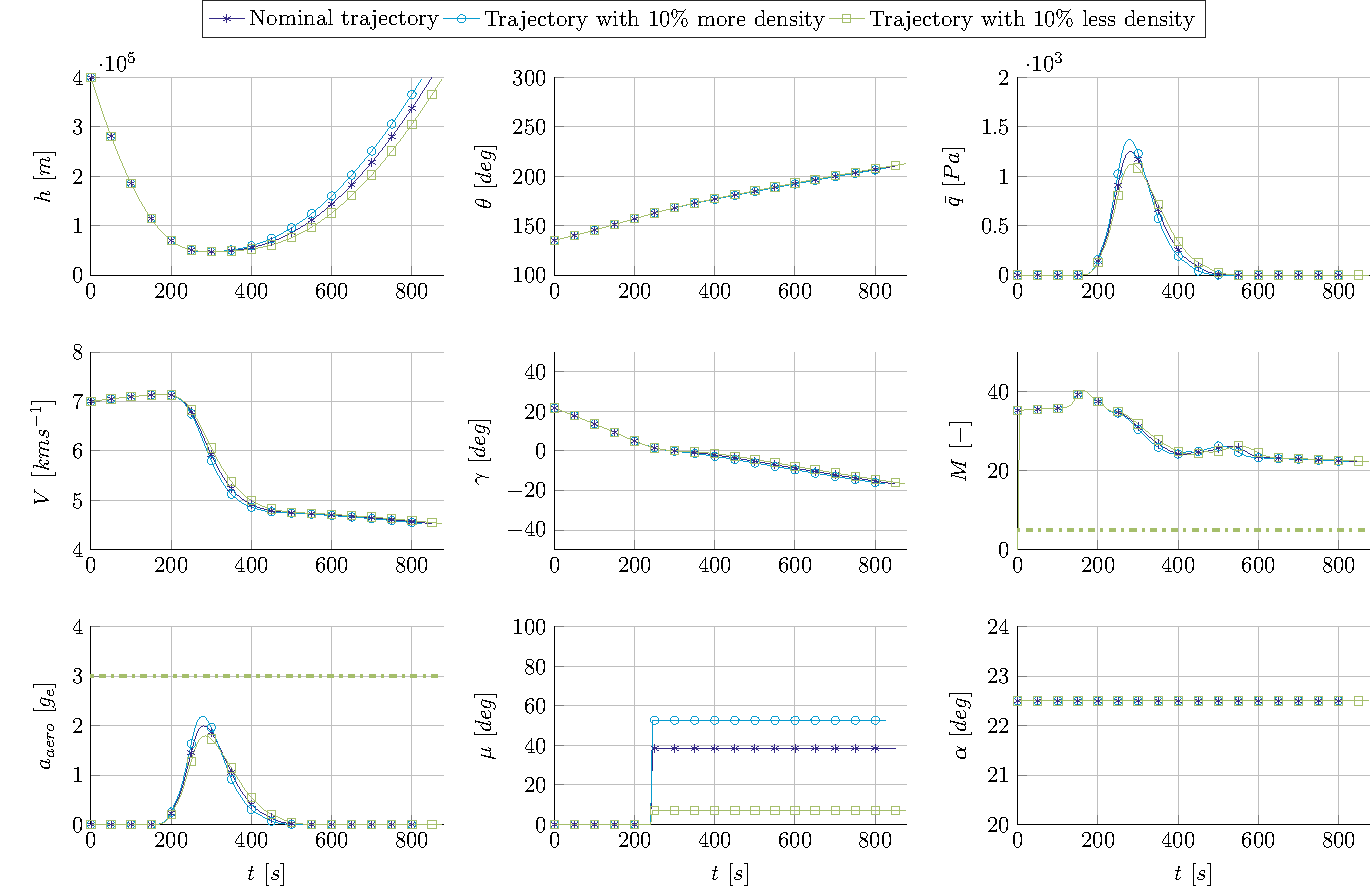
\includegraphics[width=0.99\textwidth]{Figure/Orbit/sensitivity_aerocapture.pdf}
	\caption{Results of the aerocapture trajectory for three different density profiles. The trajectories with modified density are corrected (changed \gls{sym:mu} profile) to maintain the same exit velocity. The horizontal dashed lines are design limits (for the \gls{sym:M} and \gls{sym:acc} plots) }
	\label{fig:orbit_aerocapture_data}
\end{sidewaysfigure}

\paragraph{Parking orbit}
***Use of orbit, extrension of time***\\
***Orbital period, 1 sol***\\

\paragraph{Entry and descent}
***Entry conditions imposed by aerocapture and parking orbit***
***trajectory based on 3g requirement \& Mach 5 reuirement***
***$\alpha$ control not nessesary***

***Sensitivity to density change +-10\% and possibility to correct for it***\\
\begin{sidewaysfigure}
	\centering
	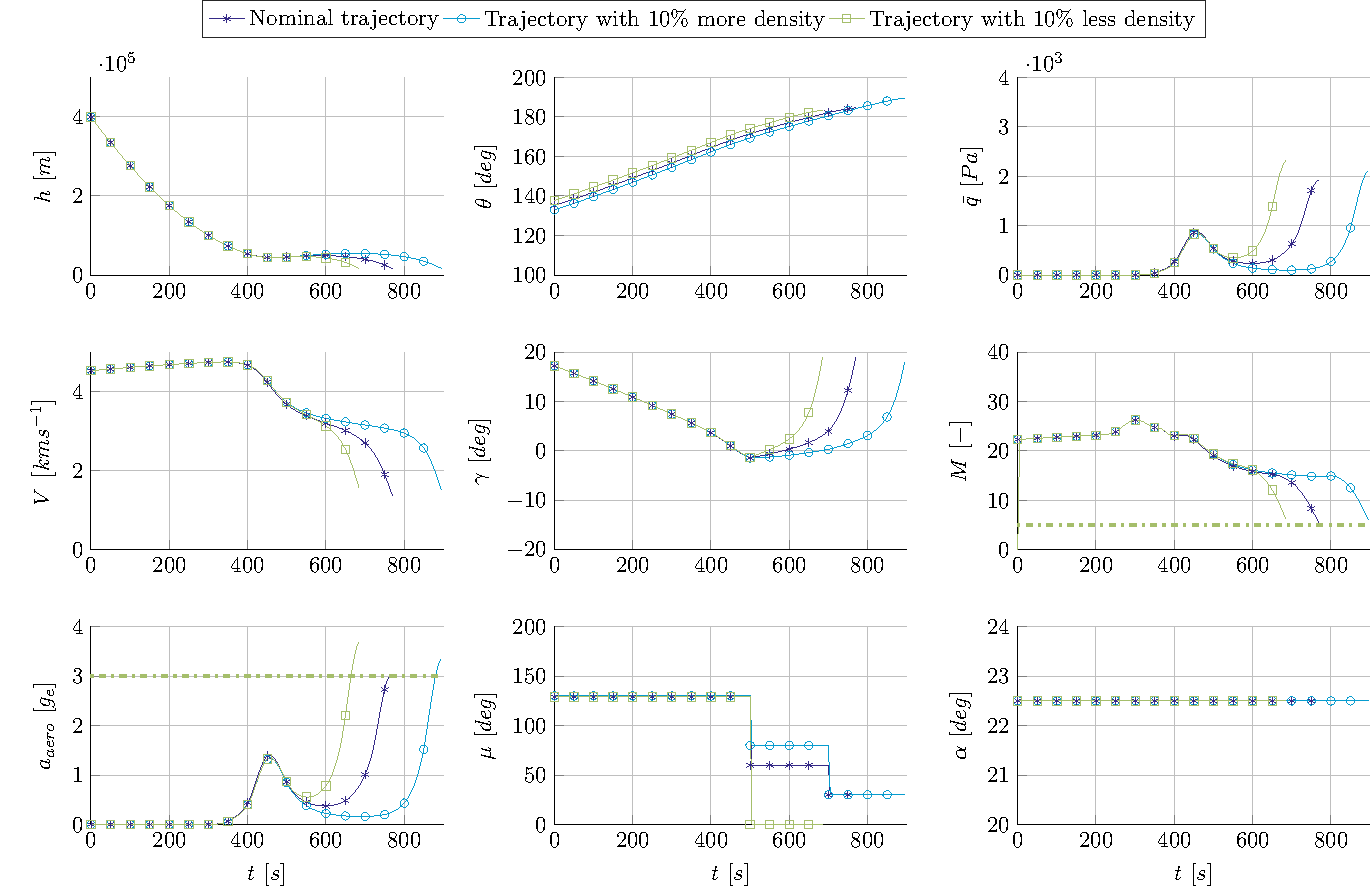
\includegraphics[width=0.99\textwidth]{Figure/Orbit/sensitivity_entry.pdf}
	\caption{Results of the re-entry trajectory for three different density profiles. The trajectories with modified density are corrected (changed \gls{sym:mu} profile) to show the ability to reach the desired landing location. The horizontal dashed lines are design limits (for the \gls{sym:M} and \gls{sym:acc} plots)}
	\label{fig:orbit_entry_data}
\end{sidewaysfigure}

\begin{figure}[h]
	\centering
	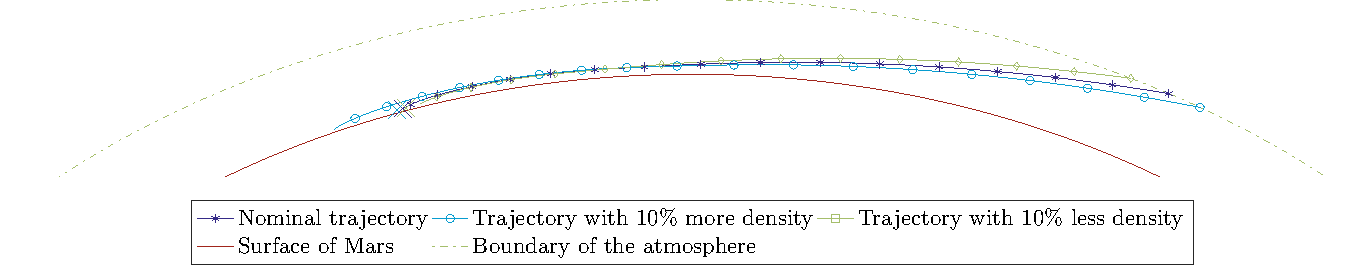
\includegraphics[width=0.99\textwidth]{Figure/Orbit/entry_mars.pdf}
	\caption{The re-entry trajectory for three different density profiles. The trajectories with modified density are corrected (changed \gls{sym:mu} profile) to show the ability to reach the desired landing location.}
	\label{fig:entry_mars}
\end{figure}
